%%%%%%%%%%%%%%%%%%%%%%%%%%%%%%%%%%%%%%%%%%  不使用 authblk 包制作标题  %%%%%%%%%%%%%%%%%%%%%%%%%%%%%%%%%%%%%%%%%%%%%%
%-------------------------------PPT Title-------------------------------------
\title{模型微调简介}
%-----------------------------------------------------------------------------

%----------------------------Author & Date------------------------------------
\author[]{\vskip +10pt 姜\;\;骏\inst{}} %[]{} (optional, use only with lots of authors)
%% - Give the names in the same order as the appear in the paper.
%% - Use the \inst{?} command only if the authors have different
%%   affiliation.
\institute[BCC]{\inst{}%
%\institute[Gain~Strong]{\inst{}%
\vskip -15pt 北京市计算中心}
%\vskip -20pt {\large 格致斯创~科技}}
\date[\today] % (optional, should be abbreviation of conference name)
{	{\fontsize{6.2pt}{4.2pt}\selectfont{\textcolor{blue}{E-mail:~}\url{jiangjun@bcc.ac.cn}}}
\vskip 45 pt {\fontsize{8.2pt}{6.2pt}\selectfont{%清华大学\;\;物理系% 报告地点
	\vskip 5 pt \textrm{2025.02}}}
}

%% - Either use conference name or its abbreviation
%% - Not really information to the audience, more for people (including
%%   yourself) who are reading the slides onlin%%   yourself) who are reading the slides onlin%%   yourself) who are reading the slides onlineee
%%%%%%%%%%%%%%%%%%%%%%%%%%%%%%%%%%%%%%%%%%%%%%%%%%%%%%%%%%%%%%%%%%%%%%%%%%%%%%%%%%%%%%%%%%%%%%%%%%%%%%%%%%%%%%%%%%%%%

\subject{}
% This is only inserted into the PDF information catalog. Can be left
% out.
%\maketitle
\frame
{
%	\frametitle{\fontsize{9.5pt}{5.2pt}\selectfont{\textcolor{orange}{“高通量并发式材料计算算法与软件”年度检查}}}
\titlepage
}
%-----------------------------------------------------------------------------

%------------------------------------------------------------------------------列出全文 outline ---------------------------------------------------------------------------------
\section*{}
\frame[allowframebreaks]
{
	\frametitle{\textrm{Outline}}
%  \frametitle{\textcolor{mycolor}{\secname}}
  \tableofcontents%[current,currentsection,currentsubsection]
}
%在每个section之前列出全部Outline
%类似的在每个subsection之前列出全部Outline是\AtBeginSubsection[]
%\AtBeginSection[]
%{
%  \frame<handout:0>%[allowframebreaks]
%  {
%    \frametitle{Outline}
%%全部Outline中,本部分加亮
%    \tableofcontents[current,currentsection]
%  }
%}

%-----------------------------------------------PPT main Body------------------------------------------------------------------------------------
\small
\section{大模型微调}
% 大模型微调的基本概念
\begin{frame}
    \frametitle{通用大模型}
    \textcolor{red}{通用大模型:}~{\fontsize{8.2pt}{6.2pt}\selectfont{如\textrm{GPT}、\textrm{LLaMA}、\textrm{DeepSeek}}}
\begin{figure}[h!]
\vspace*{-0.05in}
\centering
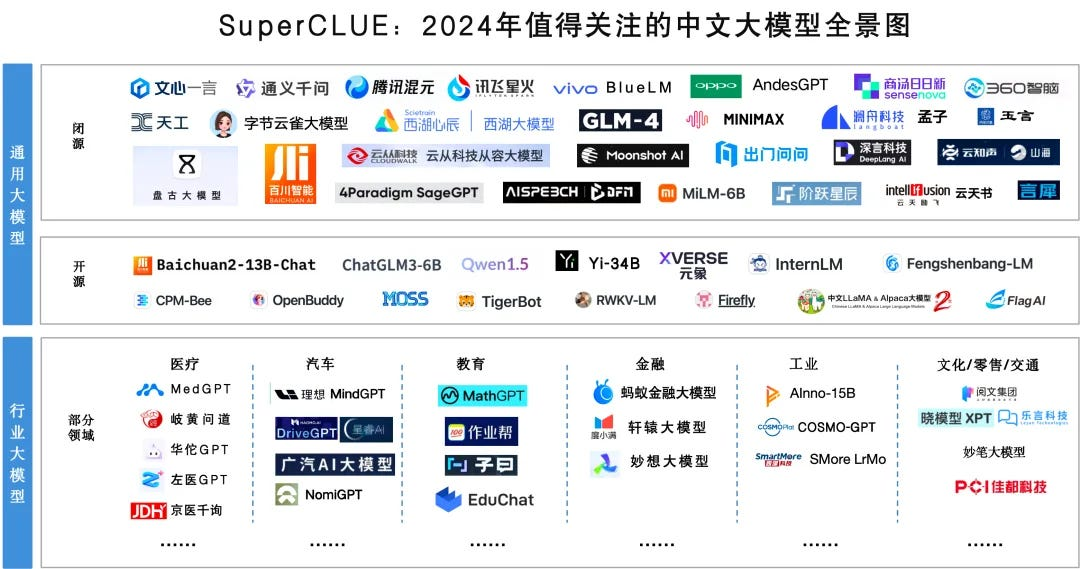
\includegraphics[height=2.0in, width=4.0in, viewport=0 0 1080 510,clip]{Figures/LLM_model-logo_Chinese.jpg}
%\caption{\tiny \textrm{Pseudopotential for metallic sodium, based on the empty core model and screened by the Thomas-Fermi dielectric function.}}%(与文献\cite{EPJB33-47_2003}图1对比)
\label{LLM_model-logo_Chinese}
\end{figure}
\textcolor{blue}{具备强大的通用知识和语言理解能力,预训练参数规模巨大}
\end{frame}

\begin{frame}
    \frametitle{大模型的微调}
通用模型在特定领域存在局限性
         **为什么要微调**:~微调能适配特定任务或领域,提升特定场景性能,如法律文书分析、医疗诊断助手
         **微调的定义**:~在预训练模型基础上,通过特定数据集训练,调整部分或全部参数,以适应特定任务或领域
\begin{figure}[h!]
\vspace*{-0.05in}
\centering
\includegraphics[height=2.0in, width=4.0in, viewport=0 0 1080 510,clip]{Figures/.jpg}
%\caption{\tiny \textrm{Pseudopotential for metallic sodium, based on the empty core model and screened by the Thomas-Fermi dielectric function.}}%(与文献\cite{EPJB33-47_2003}图1对比)
\label{LLM_model-fine_tuning}
\end{figure}
\end{frame}

\section{方法、工具与流程}
\subsection{大模型微调的方法}
% 大模型微调的方法
\begin{frame}
    \frametitle{大模型微调的方法}
    \begin{itemize}
        \item **基于特征提取的微调**:冻结预训练模型大部分层,仅训练新添加分类器或回归层,适用于数据量小、任务与预训练任务相关性高的场景,如图像分类任务
        \item **全模型微调**:对预训练模型所有参数进行微调,适用于数据量充足、任务与预训练任务差异大的场景,如情感分析任务
        \item **部分层微调**:选择预训练模型部分层进行微调,平衡训练成本和模型性能,如文本摘要任务
    \end{itemize}
%    \begin{center}
%        \includegraphics[width=0.8\textwidth]{微调方法流程图}
%    \end{center}
\end{frame}

\subsection{大模型微调的工具}
% 大模型微调的工具
\begin{frame}[fragile,allowframebreaks]
    \frametitle{大模型微调的工具}
    \begin{columns}[c]
        \column{0.33\textwidth}
%            \centerline{\includegraphics[width=0.8\textwidth]{HuggingFace图标}}
            \textbf{Hugging Face Transformers}:提供丰富预训练模型、简单易用API,支持多种深度学习框架
            \begin{lstlisting}[style=pythonstyle]
# Hugging Face微调示例代码
from transformers import AutoModelForSequenceClassification
from transformers import TrainingArguments, Trainer
model = AutoModelForSequenceClassification.from_pretrained("bert-base-uncased", num_labels = 2)
# 后续训练代码
            \end{lstlisting}
        \column{0.33\textwidth}
%            \centerline{\includegraphics[width=0.8\textwidth]{TFX图标}}
            \textbf{TensorFlow Extended (TFX)}:支持端到端模型开发和部署,提供数据预处理、模型训练、评估和部署等功能
%            \includegraphics[width=0.8\textwidth]{TFX微调工作流程图}
        \column{0.33\textwidth}
%            \centerline{\includegraphics[width=0.8\textwidth]{PyTorchLightning图标}}
            \textbf{PyTorch Lightning}:简化PyTorch模型训练过程,提高代码可维护性和可扩展性
            \begin{lstlisting}[style=pythonstyle]
# PyTorch Lightning微调示例代码
from pytorch_lightning import LightningModule

class MyModel(LightningModule):

     def __init__(self):
         super().__init__()
  # 模型定义
    def training_step(self, batch, batch_idx):
  # 训练步骤
  # 后续训练代码
            \end{lstlisting}
    \end{columns}
%    \begin{center}
%        \begin{tabular}{|c|c|c|}
%            \hline
%            工具 & 特点 & 适用场景 \\
%            \hline
%            Hugging Face Transformers & 丰富模型、易用API & 快速原型开发 \\
%            \hline
%            TensorFlow Extended (TFX) & 端到端开发 & 大规模生产场景 \\
%            \hline
%            PyTorch Lightning & 简化训练 & PyTorch开发者 \\
%            \hline
%        \end{tabular}
%    \end{center}
\end{frame}

\subsection{大模型微调的步骤}
% 大模型微调的实现步骤
\begin{frame}[fragile,allowframebreaks]
    \frametitle{大模型微调的实现步骤}
    \begin{enumerate}
        \item **数据准备**:收集标注特定领域数据,进行清洗和预处理,划分训练集、验证集和测试集
            \begin{lstlisting}[style=pythonstyle]
import pandas as pd
data = pd.read_csv('data.csv')
# 数据清洗和划分代码
            \end{lstlisting}
        \item **模型选择**:根据任务需求和数据特点选择预训练模型,考虑模型大小、性能和可扩展性优先选择任务适配、参数规模合适的模型
        \item **微调配置**:设置训练参数,如学习率、批量大小、训练轮数,选择优化器和损失函数
            \begin{lstlisting}[style=pythonstyle]
from torch.optim import Adam
optimizer = Adam(model.parameters(), lr = 0.001)
# 损失函数和其他配置代码
            \end{lstlisting}
        \item **模型训练**:在训练集上微调模型,监控性能指标,如准确率、损失值
            \begin{lstlisting}[style=pythonstyle]
for epoch in range(num_epochs):
    model.train()
    # 训练步骤和指标监控代码
            \end{lstlisting}
            \begin{center}
%                \includegraphics[width=0.8\textwidth]{训练曲线}
            \end{center}
        \item **模型评估**:在验证集和测试集上评估微调后模型性能,分析评估结果
            \begin{lstlisting}[style=pythonstyle]
model.eval()
# 评估代码和指标计算
            \end{lstlisting}
    \end{enumerate}
    \begin{center}
%        \includegraphics[width=0.8\textwidth]{微调实现步骤图}
    \end{center}
\end{frame}

% 案例分析
\begin{frame}[allowframebreaks]
    \frametitle{案例分析}
    \begin{enumerate}
        \item
            \textbf{电商领域:商品推荐模型}
            \begin{itemize}
                \item **案例背景**:目标是提高推荐准确率和用户点击率
                \item **数据处理**:收集商品信息、用户行为数据,标注用户偏好,处理缺失值和异常值,数据具有高维度、稀疏性特点
                \item **模型选择与微调**:选择基于Transformer的预训练模型,采用全模型微调方法设置学习率0.001,批量大小64,训练轮数10训练后模型在验证集上准确率提升10%
                \item **效果评估**:在测试集上,推荐准确率达到80%,用户点击率提高20%,但对新用户和新商品推荐效果有待提升
            \end{itemize}
        \item
            \textbf{医疗领域:市太和医院素问医疗大模型}
            \begin{itemize}
                \item **案例背景**:市太和医院将DeepSeek与自研的素问医疗大模型深度融合,实现诊疗全流程智能化落地应用
                \item **数据处理**:模型充分学习海量医疗指南、医学书籍等专业资料,并经千万量级临床案例指导
                \item **模型选择与微调**:融合DeepSeek推理技术,兼顾系统能力和效率
                \item **效果评估**:诊前,患者等待时间和医生问诊时间大幅缩短;诊中,辅助医生完成诊疗记录、鉴别诊断等工作,保障诊疗质量;诊后,帮助患者实现智能化健康管理如市民张女士通过该模型,仅30分钟就确诊为胆囊结石并制定出微创方案,诊疗效率比普通门诊提升50%以上
            \end{itemize}
        \item
            \textbf{金融领域:江苏银行DeepSeek模型应用}
            \begin{itemize}
                \item **案例背景**:江苏银行依托“智慧小苏”大语言模型服务平台,部署并微调DeepSeek-VL2多模态模型和轻量级的DeepSeek-R1推理模型
                \item **数据处理**:对海量金融数据进行深度挖掘与分析
                \item **模型选择与微调**:部署并微调DeepSeek系列模型,适配金融业务场景
                \item **效果评估**:为业务发展注入新动力,在复杂推理场景下实现人工智能技术应用,提升工作效率和服务质量
            \end{itemize}
        \item
            \textbf{工业领域:奇智孔明工业大模型}
            \begin{itemize}
                \item **案例背景**:创新奇智推出奇智孔明工业大模型2.0版本及多款大模型原生应用,参数量级达750亿以上,且通过中国信通院可信AI工业大模型评测
                \item **数据处理**:助力打通AI大模型与传统工业生产的壁垒
                \item **模型选择与微调**:持续投入研发升级模型
                \item **效果评估**:推出“ChatCAD生成式辅助工业设计”“ChatRobot生成式工业机器人调度”等应用前者可通过对话生成工业设计图,后者能实现对工业机器人的意念操控 
            \end{itemize}
        \item
            \textbf{凝聚态物理与材料科学领域:文献抽取模型}
            \begin{itemize}
                \item **案例背景**:凝聚态物理和材料科学文献中包含大量专业术语和复杂知识,从这些文献中提取关键信息,对科研工作的开展具有重要意义但通用大模型在处理这类专业文献时,准确率和召回率较低,无法满足科研人员的需求
                \item **数据处理**:研究团队收集了大量凝聚态物理和材料科学领域的学术论文、研究报告等文献,并对其进行标注,构建了包含材料结构、物理性质、实验方法、研究结论等信息的数据集随后对数据进行清洗,去除噪声数据和重复数据,并按照8:1:1的比例划分为训练集、验证集和测试集
                \item **模型选择与微调**:团队选择了在自然语言处理领域表现优异的BERT模型作为预训练模型,并采用全模型微调方法设置学习率为0.0001,批量大小为32,训练轮数为10借助Hugging Face Transformers工具,简化微调过程
                \item **效果评估**:微调后的模型在测试集上,关键信息的抽取准确率从通用模型的60%提升到了85%,召回率从50%提升到了75%,大幅提高了文献分析的效率和准确性,帮助科研人员快速获取所需信息,加速科研创新进程
            \end{itemize}
    \end{enumerate}
\end{frame}

\section{效果与评价}
% 大模型微调的效果评价
\begin{frame}
    \frametitle{大模型微调的效果评价}
    \begin{itemize}
        \item **性能提升显著**:微调能让模型在特定任务上表现远超通用模型,如在电商推荐、医疗诊断、金融服务、工业设计以及凝聚态物理和材料文献抽取等案例中,相关模型的准确率、效率等性能指标显著提高
        \item **灵活性与适应性增强**:通过微调,一个预训练大模型可适配多种不同领域和任务,降低模型开发的时间和资源成本,例如同一基础模型经微调后,可同时用于多个不同场景
        \item **数据需求与成本考量**:尽管微调能在较小数据集上进行,但高质量的特定领域数据仍不可或缺同时,全模型微调计算成本高,部分层微调或基于特征提取的微调虽能降低成本,却可能限制模型性能的提升幅度
        \item **潜在风险**:微调过程可能导致模型过拟合特定数据集,降低模型的泛化能力此外,不当的微调还可能放大数据中的偏差,引发公平性和安全性问题
    \end{itemize}
\end{frame}

%% 总结与展望
%\begin{frame}
%    \frametitle{总结与展望}
%    \begin{itemize}
%        \item **总结**:回顾大模型微调基本概念、方法、工具和实现步骤,大模型微调对定制化AI开发至关重要
%        \item **展望**:未来大模型微调将发展更高效方法、降低计算成本、拓展应用场景鼓励大家在实际工作中应用该技术
%    \end{itemize}
%    \begin{center}
%   %     \includegraphics[width=0.8\textwidth]{启发性图表}
%    \end{center}
%\end{frame}
